% Warum Datenklassifizierung? 
Unternehmen setzen immer mehr auf cloudbasierte SaaS-Produkte, anstatt diese selbst installieren und verwalten zu müssen \cite{Gartner.2023}. In ihrem Tagesgeschäft verlassen sich Unternehmen oft auf mehrere Softwareprodukte, um unterschiedliche Anforderungen zu erfüllen. Das führt dazu, dass Unternehmensdaten über verschiedene Applikationen und Cloud-Plattformen verteilt sind. Die Herausforderung besteht darin, den Überblick zu behalten und zu wissen, wo sich die sensiblen Daten befinden. Das Sammeln und Identifizieren von Daten in DLP-Systemen stellt aufgrund von Verschlüsselung, verborgenen Kanälen, nicht unterstützten Datenformaten und großer Mengen an Daten eine große Herausforderung dar \cite{Hauer.2015}.

\subsection{Erkennung von sensiblen Daten}
Die Methoden zur Erkennung und Klassifizierung von sensiblen Daten unterscheiden sich je nach Art und Format der Daten, sowie deren Zustand. Außerdem gibt es die Möglichkeit, Daten manuell oder automatisiert zu klassifizieren.

\subsubsection{Eigenschaften von Daten}
% Art -> welche Kategorien
Sensible Daten sind nahezu in jedem Aspekt unseres persönlichen und beruflichen Lebens präsent. Das Spektrum dieser sensiblen Informationen reicht von persönlichen Daten über Finanzinformationen und Geschäftsgeheimnissen bis hin zu biometrischen Merkmalen. Guo, Liu et al. \cite{Guo.2021} kategorisieren beispielsweise Daten in vier Bereiche:
\begin{itemize}
    \item Persönliche Informationen (z.B. Name, Geburtsdatum oder Gesundheitsinformationen)
    \item Informationen zur Netzwerkidentität (z.B. IP-Adresse, MAC-Adresse oder E-Mail)
    \item Vertrauliche und Anmeldeinformationen (z.B. Login-Passwort-Kombinationen, API-Token oder digitale Zertifikate)
    \item Finanzinformationen (z.B. Bankkontodaten, Kreditkarteninformationen oder Verbrauchsdaten)
\end{itemize}
Die Kategorisierung und der Detailgrad können je nach Unternehmen variieren.

Zusätzlich zu den Kategorien muss auch der Kontext berücksichtigt werden, in dem eine Information verwendet wird. Der Kontext hat direkten Einfluss auf die Sensibilität. Pogiatzis und Samakovitis \cite{Pogiatzis.2020} leiten vier verschiedene Kontextklassen ab, die auf der Bedeutung, der Interaktion, der Priorität und der Präferenz basieren, die mit jeder Information verbunden sind.

\begin{itemize}
    \item Der semantische Kontext entsteht auf Grundlage der semantischen Bedeutung eines Begriffs. Die semantische Bedeutung einer Sequenz wirkt sich also auch auf ihre Sensibilität aus.
    \item Im Kontext der Akteure hängt die Sensibilität von Daten von den Akteuren ab, die an der Informationsübermittlung beteiligt sind. Die Sensibilität wird durch die Beziehung zwischen den beteiligten Akteuren bestimmt. Zum Beispiel ist der Austausch von Gesundheitsinformationen zwischen Patient und Arzt nicht sensibel, außerhalb dieser Gruppe von Akteuren jedoch schon.
    \item Der zeitliche Kontext bezieht sich auf die Priorität der Informationen, die die Bedeutung des Begriffs beeinflussen. Eine Zeichenfolge, die als Passwort eingegeben wird, gilt bspw. als vertraulicher als wenn sie als Benutzername eingegeben wird.
    \item Der Selbstkontext wird durch die persönlichen Präferenzen des Nutzers in Bezug auf seine Privatsphäre bestimmt. Zum Beispiel kann eine Person ihre ethnische Herkunft als vertrauliche Information betrachten, eine andere nicht.
\end{itemize}
Auch hier können verschiedene kontextuelle Kategorien unterschieden oder definieren werden. Zudem sind sie nicht immer klar trennbar und schließen sich nicht gegenseitig aus. Ein oder mehrere Kontexte können gleichzeitig unterschiedlich auf die Sensibilität wirken. Manche Daten können jedoch auch unabhängig vom Kontext vertraulich sein, wie z.B. Passwörter oder Kreditkartennummern.

% Daten Klassen
Die Klassifizierung von Daten in verschiedene Geheimhaltungsklassen ist ein häufig verwendetes Verfahren in militärischen und behördlichen Organisationen. Militärische Anwendungen verwenden dabei Begriffe wie 'eingeschränkt', 'vertraulich', 'geheim' und 'streng geheim' \cite{Landwehr.1984}. So ist es möglich, sensible Daten noch präziser in Vertraulichkeitsstufen zu unterteilen.

% Format -> structured, unstructured
Die Klassifizierung wird auch von der Struktur der Daten beeinflusst. Über 80\% der Daten im Internet bestehen aus unstrukturierten Daten \cite{Allahyari.2017}. Unstrukturierte Daten beziehen sich in der Regel auf Informationen, die nicht in einer relationalen Datenbank gespeichert sind. Folglich gibt es kein vordefiniertes Datenmodell und die Struktur ist unregelmäßig oder unvollständig. Selbst Datenformate wie CSV, JSON oder XML, die einige organisatorische Eigenschaften haben, verfügen in der Regel nicht über ein klar definiertes Datenmodell. Im Vergleich zu strukturierten Daten ist es schwieriger, unstrukturierte Daten abzurufen, zu analysieren und zu speichern. Während Menschen unstrukturierte Daten leicht verarbeiten können, haben Maschinen oft Schwierigkeiten damit \cite{Guo.2021}.

Die Herausforderung bei der Datenklassifizierung besteht daher darin, die Kategorien, den Kontext, die Vertraulichkeitsstufen und die Struktur der Daten zu berücksichtigen.

\subsubsection{Datenzustand}
Im Bereich der Informationssicherheit werden Daten je nach ihrem Zustand unterschiedlich betrachtet. Die verschiedenen Datenzustände helfen dabei, die geeigneten Sicherheitsmaßnahmen zu bestimmen. Im Rahmen der Data Leakage Prevention können sich Daten in einem der drei Zustände befinden: Daten im Ruhezustand, Daten in Bewegung und Daten in Verwendung \cite{Shabtai.2012b}.

Daten im Ruhezustand sind solche, die auf einem physischen oder digitalen Speichermedium gespeichert sind, wie in einer Datenbank, auf einer Festplatte, im Cloud-Speicher oder einem externen Datenspeicher. Ruhende Daten sind in der Regel inaktiv, werden nicht gelesen oder übertragen. DLP-Systeme setzen für ruhende Daten Sicherheitsmaßnahmen wie Verschlüsselung, Authentifizierung und Zugriffskontrollregeln zu Erkennungs- und Überwachungszwecken ein \cite{Shishodia.2022}\cite{Shabtai.2012b}.

Daten in Bewegung beziehen sich hingegen auf den Zustand von Daten, wenn sie aktiv über Netzwerke oder andere Kommunikationskanäle übertragen werden oder sich im Speicher eines Computers befinden und zum Lesen, Aktualisieren und Verarbeiten bereit sind. Beispiele für Daten in dieser Kategorie sind Daten, die über das Internet, soziale Medien, E-Mail oder FTP/SSH übertragen werden. Daten, die über das Netzwerk übertragen werden, sollten mit Verschlüsselungsmethoden wie HTTPS, SSL oder TLS geschützt werden. DLP-Systeme nutzen Erkennungs- und Überwachungsfunktionen, um den Datenfluss durch das Netzwerk zu identifizieren und zu überwachen \cite{Shishodia.2022}\cite{Shabtai.2012b}.

Daten in Verwendung sind solche, die aktiv von einer Person oder einem System verarbeitet, aktualisiert, anhängt oder gelöscht werden. Diese Daten befinden sich auf dem Laptop, dem USB-Stick oder der externen Festplatte des Endnutzers sowie auf Netzlaufwerken oder Druckern. Da diese Daten aktiv manipuliert werden, sind sie besonders anfällig für Sicherheitsbedrohungen. Sie werden über verschiedene Endpunkte hinweg sichtbar, wenn darauf zugegriffen wird. Um diese Daten zu schützen, implementiert das DLP-System starke Benutzerauthentifizierung sowie ein Identitäts- und Profilmanagement. Je nach DLP-Technologie kann auch ein Endpunkt-Agent auf dem Gerät des Endnutzers installiert werden, um die Datennutzung und -übertragung zu überwachen \cite{Shishodia.2022}\cite{Shabtai.2012b}.

Die Unterscheidung zwischen den drei Zuständen von Daten - in Ruhe, in Bewegung und in Verwendung - ist entscheidend für die Identifizierung sensibler Informationen und die Klassifizierung von Daten. Durch die Berücksichtigung der Datenzustände können sensible Daten differenziert betrachtet und klassifiziert werden.

\subsection{Herausforderungen in der Datenklassifizierung}
% Warum manuell
In der Literatur wurden verschiedene Studien durchgeführt, um Klassifizierungsmethoden zur Gewährleistung der Datensicherheit in der Cloud zu untersuchen. Die vorgeschlagenen Lösungen lassen sich in manuelle und automatische Klassifizierung unterteilen. Bei der manuellen Klassifizierung werden die Klassen durch eine Person festgelegt und bei der automatische Klassifizierung werden dafür Algorithmen eingesetzt. Obwohl automatisierte Technologien Fortschritte machen, bleibt die manuelle Datenklassifizierung, insbesondere für sensible Informationen wie geistiges Eigentum, weit verbreitet. Trotz ihres Potenzials für umfassende Berücksichtigung von Datenkontexten und -zuständen birgt die manuelle Klassifizierung Risiken wie menschliche Fehler und Inkonsistenzen. Zudem kann sie bei großen Datenmengen zeitaufwändig werden und die Anpassungsfähigkeit beeinträchtigen \cite{Venhorst.2019}. Angesichts des wachsenden Datenvolumens erscheint die automatisierte Datenklassifizierung als effizientere Lösung für präzise und konsistente Identifizierung sensibler Daten.

% ###########################################
% warum automatisiert
Die automatische Datenklassifizierung bezeichnet den Prozess, bei dem maschinelle Algorithmen und Technologien verwendet werden, um Daten automatisch zu identifizieren, zu kategorisieren und entsprechend ihrer Sensitivität zu klassifizieren. Diese Methode nutzt maschinelles Lernen, Mustererkennung oder künstliche Intelligenz, um Daten zu analysieren und automatisch passende Klassifizierungen zuzuweisen.

Aktuelle Techniken in der Data Leakage Prevention lassen sich im Allgemeinen in zwei Kategorien unterteilen: inhaltsbasierte Analyse und kontextbasierte Analyse. Inhaltsbasierte Methoden untersuchen den Dateninhalt anhand von Merkmalen sensibler Informationen. Sie nutzen vorhersehbare Muster wie bspw. IP-Adressen, E-Mail-Adressen oder bestimmte Wörter, um sensible Daten zu erkennen. Kontextbasierte Techniken identifizieren vertrauliche Daten anhand von Merkmalen im Zusammenhang mit den überwachten Daten. Der kontextbasierte Ansatz ist somit effektiver für vertrauliche Daten ohne vorhersehbare Muster \cite{Kuzina.2023}.

%Tabelle mit content-based vs. context-based
\begin{table}[htbp]
    \normalsize
    \caption{Methoden der automatischen Datenklassifizierung. Quelle: eigene Darstellung.}
    \label{t:methoden}
    \begin{center}
        \begin{tabulary}{15cm}{|L|L|}
            \hline
            \textbf{Kategorie} & \textbf{Methode} \bigstrut  \\
            \hline
            \hline
            \multirow{4}{*}{inhaltsbasiert} & regelbasierte Methoden \bigstrut[t]     \\
            & Data Fingerprinting               \\
            & kNN              \\
            & Boosting \\
            \hline
            \multirow{3}{*}{inhalts- und kontextbasiert}  & Clusteranalyse  \bigstrut[t] \\
            & CASSED \\
            & BERT-BiLSTM \\
            \hline
        \end{tabulary}
    \end{center}
\end{table}

Um sensible Informationen umfassender und genauer zu extrahieren, sollten daher verschiedene Methoden angewendet werden. Tabelle \ref{t:methoden} zeigt die am häufigsten verwendeten Methoden in der Literatur. Die meisten kontexbasierten Ansätze kombinieren inhaltsbasierte und kontextbasierte Methoden, um die Vorteile beider Kategorien zu nutzen und die Genauigkeit der Klassifizierung zu verbessern.


% ###########################################
\subsection{Klassifizierung mit manueller Definition}
In diesem Abschnitt werden regelbasierte Methoden und Data Fingerprinting als zwei häufig verwendete Ansätze zur automatischen Datenklassifizierung vorgestellt. Eine gemeinsame Eigenschaft dieser Methoden ist, dass sie voraussetzen, dass eine Person zunächst Regeln oder ein Wörterbuch definiert, die die Methode dann zur automatischen Klassifizierung der Daten verwendet.

% ###########################################
\paragraph{regelbasierte Methoden}
% rule-based/regular-matching/Dictionary
Regelbasierte Methoden zur automatischen Datenklassifizierung verwenden im Wesentlichen ein Wörterbuch oder eine Regel, um den gegebenen Text mit einer Liste regulärer Ausdrücke und Schlüsselwörter abzugleichen. Diese Methode setzt vordefinierte Regeln und Bedingungen ein, um bestimmte Datentypen oder Muster automatisch zu identifizieren und zu klassifizieren. Diese Regeln können auf verschiedenen Merkmalen wie Schlüsselwörtern, Mustern, Dateiformaten oder spezifischen Attributen wie Datumsangaben basieren \cite{Ong.2017}.
Ein Beispiel für die Anwendung regelbasierter Methoden ist die Identifikation von Kreditkartennummern in Textdokumenten. Hier kann ein regulärer Ausdruck verwendet werden, der die Zeichenfolge nach dem Muster einer Kreditkartennummer definiert. Muster in regulären Ausdrücken umfassen normale Zeichen mit wörtlicher Bedeutung sowie Metazeichen, um ein Erkennungsmuster zu bilden \cite{Alneyadi.2016}. Der reguläre Ausdruck für die MasterCard Kreditkartennummer wäre zum Beispiel $\verb!^5[1-5][0-9]{14}$!$. Dieser Ausdruck definiert, dass alle MasterCard-Nummern mit einer 5 beginnen, dann eine Zahl zwischen 1 und 5 enthalten und anschließend eine beliebige Reihenfolge von 14 Zahlen haben.
Regeln können sich auch auf bestimmte Schlüsselwörter oder Phrasen beziehen, wie bspw. 'Sozialversicherungsnummer' oder 'vertraulich', die auf personenbezogene Informationen hinweisen können.
Der Vorteil regelbasierter Methoden liegt in ihrer klaren Struktur und der Möglichkeit, spezifische Anforderungen und Richtlinien der Organisation abzubilden. Sie ermöglichen eine präzise und konsistente Klassifizierung von Daten gemäß vordefinierten Sicherheitsstandards. Da die Klassifizierung auf klaren, vorher festgelegten Regeln basiert, ermöglichen regelbasierte Ansätze auch eine gewisse Transparenz und Nachvollziehbarkeit.
Jedoch können regelbasierte Methoden bei der Verarbeitung komplexer und sich verändernder Datenmuster weniger nützlich sein. Die Regeln werden schnell unpraktisch, wenn verschiedene Datenformate, Kontexte, Wortvariationen und Abkürzungen kombiniert werden müssen. Der effektive Einsatz dieser Methode erfordert zudem ein gut definiertes und gepflegtes Wörterbuch und Regelwerk. Außerdem wird der semantische Kontext der Wörter bei einem reinen Textabgleich nicht berücksichtigt, was zu einer geringen Genauigkeit der Klassifizierung führen kann \cite{Ong.2017}.
Trotz dieser Einschränkungen bieten regelbasierte Ansätze eine grundlegende und robuste Methode zur Sicherstellung einer konsistenten Datenklassifizierung.

% ###########################################
\paragraph{Data Fingerprinting} \label{fingerprint}
Data Fingerprinting oder auch Document Fingerprinting erstellt eindeutige Fingerabdrücke für bestimmte Datenfragmente oder ganze Dateien. Diese Fingerabdrücke dienen als eindeutige Identifikatoren für die entsprechenden Daten und werden genutzt, um sensible Daten zu identifizieren und automatisch zu klassifizieren. Anhand von Wortmustern aus regulären Ausdrücken oder vordefinierten Wörterbüchern werden benüötigte Wörter, Sätze oder ganze Dateien identifiziert und eine Auswahl an eindeutigen Fingerabdrücke dafür erstellt, die als Vorlage dienen. Diese Fingerabdrücke können dann verwendet werden, um Fingerabdrücke von nicht-klassifizierten Daten zu vergleichen und zu klassifizieren.
Häufig werden Hash-Funktionen wie MD5 oder SHA1 verwendet, um Datenfingerprints zu erstellen, die eine algorithmisch generierte Zeichenfolge fester Größe für die Daten darstellen. Die Hashes von zwei Dateien unterscheiden sich jedoch bereits, sobald nur ein Zeichen verändert wurde \cite{Alneyadi.2016}. Ein weiterer Ansatz ist deshalb das sogenannte 'Fuzzy-Hashing'. Dabei werden die Daten in Blöcken verarbeitet, wodurch die Hash-Ausgabe bei ähnlichen Daten größtenteils übereinstimmende Blöcke enthält. So kann die prozentuale Ähnlichkeit mithilfe einer mathematischen Vergleichsfunktion bestimmt werden \cite{Shu.2015}.

Das Data Fingerprinting kann sowohl im Speicher als auch bei Netzwerkübertragungen und Verwendung von Daten eingesetzt werden. Es ist jedoch wichtig zu beachten, dass der Fingerabdruck in manchen Fällen keine zuverlässige Methode ist. Die Klassifizierung funktioniert zun Beispiel nicht, wenn die Daten verschlüsselt oder passwortgeschützt sind oder wenn der Inhalt nicht eindeutig mit dem Fingerabdruck übereinstimmt. Zudem ist es notwendig, dass die Vorlagen kontinuierlich aktualisiert werden. Außerdem kann der Ansatz kann bei großen Datenmengen ressourcenintensiv sein, da die Fingerabdrücke ständig gespeichert und berechnet werden müssen.


% ###########################################
\subsection{Klassifizierung mit künstlicher Intelligenz}
% Ali Abdulsattar Jabbar, Wesam Sameer Bhaya 2023 – Security of private cloud using
Die Datenklassifizierung ist eine Technik aus dem Bereich der KI, mit der die Klassen von nicht klassifizierten Daten vorhergesagt wird. KI-Methoden lassen sich in zwei Kategorien einteilen: überwachtes Lernen und unüberwachtes Lernen. Beim überwachten Lernen sind Testdaten mit bereits zugeteilten Klassen vordefiniert. Das Modell kann seine Ergebnisse mit den Zielklassen vergleichen und von den Fehlern lernen. Im Gegensatz dazu sind beim unüberwachten Lernen keine Klassen definiert, sondern die Klassifizierung der Daten erfolgt automatisch. Ein unüberwachter Algorithmus sucht nach Mustern und Ähnlichkeiten zwischen den Elementen \cite{Frochte.2018b}.

Die meisten Methoden erfordern eine vorherige Bereinigung oder Vorbereitung der Daten, wobei die genauen Schritte je nach Methode variieren können. Der Datensatz wird meistens von Stop-Wörtern bereinigt, die keinen oder nur geringen Kontext liefern, wie bspw. 'und' oder 'der'. In der Textverarbeitung sind Stemming und Lemmatization klassische Bereinigungsmethoden. Beim Stemming werden die Wörter der Eingabe auf ihren Wortstamm zurückgeführt, während bei der Lemmatization ähnliche oder inhaltlich gleiche Begriffe vereinheitlicht werden.
Diese Schritte dienen dazu, die grammatikalische Komplexität des Inputs zu reduzieren und die Datenqualität zu optimieren. Für Methoden wie neuronale Netze müssen die Eingabedaten zusätzlich in Token und Vektoren umgewandelt werden. Bei der Tokenization wird der Text in einzelne Bestandteile, sogenannte Tokens, aufgeteilt. In der Regel sind das einzelne Worte. Die Tokens werden dann in Vektoren umgewandelt, die das jeweilige Token im Modell repräsentieren. Für die Vektorisierung gibt es verschiedene Algorithmen, um Informationen wie inhaltlich ähnliche oder zusammenhängende Tokens zu behalten \cite{Kamath.2019}.

Im Folgenden werden Klassifizierungsmethoden aus dem Bereich der künstlichen Intelligenz analysiert. Dabei wurden Methoden ausgewählt, die sich in Studien als effektiv für die automatischen Klassifizierung im Kontext der Informationssicherheit bewährt haben.


% ###########################################
\paragraph{k-NN}
% K-NN (k Nearest Neighbors)
Die Methode von Zardari, Jung et al. \cite{Zardari.2014} markiert einen Meilenstein, indem sie laut eigener Aussage als erste maschinelles Lernen zur Datenklassifizierung im Kontext des Cloud Computing einsetzen. Der Bereich des maschinellen Lernens ist eine Unterkategorie der künstlichen Intelligenz, dessen Ziel es ist, präzise Ergebnisse durch Identifizieren von Mustern zu liefern. Sie verwendeten die k-Nearest-Neighbor-Methode (k-NN), um Daten in der Cloud als sensibel und nicht-sensibel zu klassifizieren. K-NN ist ein überwachter maschineller Lernalgorithmus, der für Klassifizierung, Mustererkennung und Schätzungen verwendet wird. Diese Methode geht davon aus, dass ähnliche Dinge normalerweise nahe beieinander liegen. Die k-NN-Methode verwendet die nächsten Nachbarn eines Datenpunkts, um Vorhersagen oder Klassenzuweisungen zu treffen. Der Algorithmus beginnt mit einem Datensatz, der Beispiele mit bekannten Klassen oder Werten enthält. Die Wahl des 'k' bestimmt die Anzahl der nächsten Nachbarn. Um die Ähnlichkeit zwischen den Datenpunkten zu bestimmen, wird ein Distanzmaß wie der euklidische Abstand oder die Manhattandistanz verwendet. Sie messen den Abstand zwischen den Merkmalsvektoren der Datenpunkte. Für einen gegebenen Datenpunkt werden die k nächsten Nachbarn basierend auf dem berechneten Distanzmaß aus dem Datensatz ausgewählt. Bei der Klassifikation werden die Klassen der ausgewählten k Nachbarn betrachtet und die Mehrheitsklasse wird für den gegebenen Datenpunkt verwendet \cite{Frochte.2018b}.
% TODO: Bild?

In \cite{Zardari.2014} hat die Einteilung der Daten in zwei Klassen gut funktioniert. Doch die Wahl des passenden 'k' ist bei diesem Algorithmus entscheidend. Ein zu kleines 'k' kann dazu führen, dass potenziell passende Datenpunkte ausgeschlossen werden und ein zu großes 'k' führt zu einer zu groben Klassifizierung. Abbildung \ref{f:knn} veranschaulicht die Auswirkungen der Wahl des 'k'. Je nach Größe des k wird der unbekannte Punkt (roter Stern) entweder der Klasse A oder der Klasse B zugeordnet. Aufgrund der Verwendung aller Trainingsdaten ist zudem die Rechenkomplexität bei diesem Algorithmus hoch, da bei jeder Vorhersage der Abstand berechnet und die gesamten Trainingsdatendistanzen sortiert werden müssen. Außerdem ist die Mehrheitsentscheidung bei der Klassifizierung nicht immer die optimale Methode, da je nach Anzahl der Nachbarn die Abstände stark variieren können und trotzdem immer alle gewählten Nachbarn berücksichtigt werden.

\begin{figure}[htbp]
    \centering
    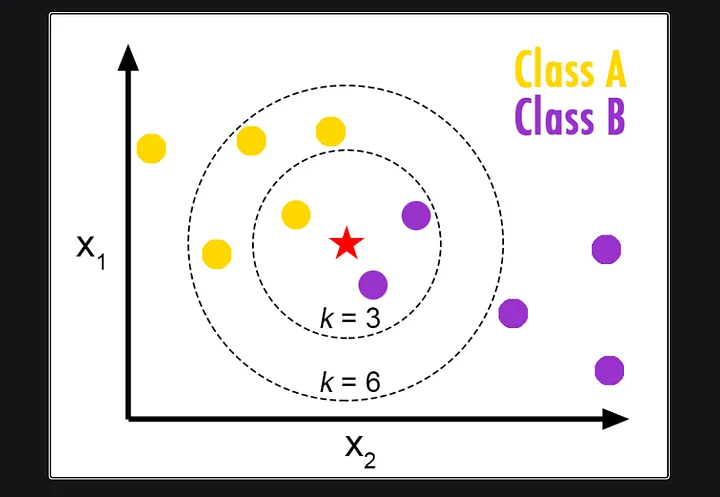
\includegraphics[width=0.7\linewidth]{\figdir/knn.png}
    \caption{Einfluss des gewählten 'k'. Quelle: \cite{Shah.03.03.2021}.}
    \label{f:knn}
\end{figure}


% ###########################################
\paragraph{Boosting}
Ensemble Learning ist ein Begriff aus dem maschinellen Lernen und beschreibt das Zusammenschalten von mehreren Methoden, um das Modellergebnis zu verbessern. Boosting ist ein Ensemble-Learning-Ansatz, der mehrere schwache Modelle zu einem starken Modell zusammenzusetzt \cite{Frochte.2018c}.
Kaur, Zandu \cite{Kaur.2016} schlagen für die Klassifizierung von sensiblen Daten eine neue Boosting-Architektur vor. Als Klassifikator wird eine Kombination aus dem Naive Bayes Klassifikator und AdaBoost verwendet. Der Naive Bayes Algorithmus ist eine Klassifizierungsmethode, die auf dem  Bayes'schen Theorem beruht. Die Grundlage ist die Annahme, dass das Auftreten eines Merkmals unabhängig vom Auftreten eines anderen Merkmals innerhalb der Klasse ist. Das  Bayes'sche Theorem ist eine Formel zur Berechnung der bedingten Wahrscheinlichkeit ${P(A|B)}$, also der Wahrscheinlichkeit von A unter der Bedingung von B. Diese bedingte Wahrscheinlichkeit lässt sich mit der Formel \ref{e:naive-bayes} berechnen. Diese Methode ermöglicht die Klassifizierung eines Merkmals, indem für jede Klasse berechnet wird, mit welcher Wahrscheinlichkeit das Merkmal zu dieser Klasse gehört. Die Zuordnung erfolgt dann basierend auf der höchsten Wahrscheinlichkeit. \cite{Frochte.2018d}.

\begin{equation}
    \label{e:naive-bayes}
    P(A|B) = \frac{P(B|A) * P(A)}{P(B)}
\end{equation}

Im Ansatz von \cite{Kaur.2016} wird der Klassifikator mit AdaBoost optimiert, einer Abkürzung für adaptive Boosting. AdaBoost kombiniert mehrere schwache Klassifikatoren zu einem starken Klassifikator. Dabei werden iterativ mehrere Klassifikatoren hinzugefügt und der Datensatz stetig neu gewichtet, damit sich der nächste Klassifikator auf die Fehler des vorherigen Klassifikators konzentriert \cite{Frochte.2018c}.

In der neuen Klassifikationsmethode von \cite{Kaur.2016} wird der Trainingsdatensatz zuerst in eine bestimmte Anzahl von Teildatensätzen aufgeteilt. Anschließend werden die einzelnen Teildatensätze schrittweise verarbeitet. Jeder Teildatensatz enthält eine Menge an Datentupeln, also eine Menge an Wörtern oder Sätzen. Zu Beginn erhält jedes Tupel die gleiche Gewichtung. Dann wird das hybride Klassifizierungsmodell aus Naive Bayes und AdaBoost mit dem Teildatensatz trainiert. Anschließend werden die Gewichte der Tupel aktualisiert, je nachdem ob sie richtig oder falsch klassifiziert wurden. Nach den Durchgängen aller Teildatensätze ergibt sich ein Set an Klassifikator-Modellen mit jeweiligen Gewichtungen, die in Kombination genaue Vorhersagen für Klassen treffen.

Kaur, Zandu \cite{Kaur.2016} zeigten, dass ihre vorgeschlagene Methode mit 94,2529\% Genauigkeit deutlich besser klassifiziert als der k-NN-Algorithmus, der nur eine Genauigkeit von 51,7241\% hatte.

% ###########################################
\paragraph{Clusteranalyse}
% auf Basis von wenigen manuell klassifizierten Daten können Cluster gebildet werden
Die Clusteranalyse ist eine Datenanalysetechnik aus dem Bereich des maschinellen Lernens. Clustering ist eine unüberwachte Lernmethode, die Muster in Eingabedaten ohne vordefinierte Zielwerte erkennt. Bei der Clusteranalyse werden unsortierte Informationen auf der Grundlage von Ähnlichkeiten, Mustern und Unterschieden gruppiert, ohne dass die Daten zuvor trainiert wurden. Im Kontext der Klassifizierung sensibler Daten wird die Clusteranalyse auf die Daten in einem Unternehmen angewendet. Die resultierenden Cluster enthalten dann ähnliche Dokumente nach einer Ähnlichkeitsmetrik wie dem euklidischen Abstand oder der Kosinusähnlichkeit \cite{Suyal.2014}.
Um die Clusteranalyse als Klassifikator zu nutzen, müssen vor der Analyse relevante Merkmale oder Attribute definiert werden, um sensible Daten zu identifizieren. Anschließend können die Cluster anhand der Merkmale klassifiziert werden.

Zwei gängige Clustering-Methoden sind das hierarchische Clustering und das partitionierende Clustering. Hierarchisches Clustering wird in der Regel für das Clustering von Texten verwendet, wobei jedes Dokument auf der Grundlage seiner Ähnlichkeit schrittweise in einen vordefinierten Cluster zusammengeführt wird. Durch diesen Prozess entsteht eine Clusterhierarchie, die als Baumstruktur, das sogenannte Dendrogramm, dargestellt werden kann. Abbildung \ref{f:clustering_daten} zeigt einen Beispieldatensatz mit den Objekten 'a' bis 'f'. In diesem Datensatz liegen die Objekte 'b' und 'c' sowie 'd' und 'e' sehr nahe beieinander. Der Clustering-Algorithmus fasst nach und nach die Objekte mit dem geringsten Abstand zusammen, gefolgt von den nächstgelegenen Objekten oder Clustern, bis der gesamte Datensatz gruppiert ist. So entsteht ein Baum wie in Abbildung \ref{f:clustering_baum}, bei dem die Blätter Cluster darstellen, die nur ein einzelnes Objekt aus dem Datensatz enthalten, und die Wurzel einen einzelnen Cluster, der alle Objekte enthält. Die Kanten zwischen den Knoten haben außerdem ein Attribut, das den Abstand zwischen den beiden Clustern angibt. Je nach gewünschter Anzahl von Clustern können die Cluster auf einer bestimmten Ebene des Baumes verwendet werden \cite{Suyal.2014}.
% TODO: Distanz Algorithmus im Detail darstellen?

\begin{figure}[htbp]
    \centering
    \begin{subfigure}[b]{0.47\linewidth}
        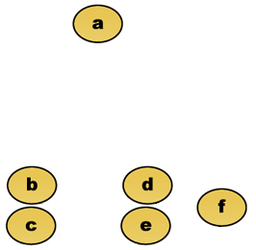
\includegraphics[width=\linewidth]{\figdir/clustering_daten}
        \caption{Datensatz. Quelle: In Anlehnung an \cite{Bonthu.2023}.}
        \label{f:clustering_daten}
    \end{subfigure}
    \hfill
    \begin{subfigure}[b]{0.47\linewidth}
        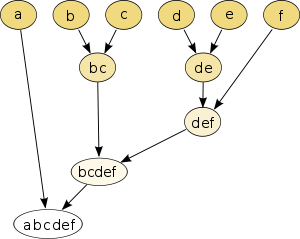
\includegraphics[width=\linewidth]{\figdir/clustering_dendrogramm}
        \caption{Dendrogramm. Quelle: In Anlehnung an \cite{Bonthu.2023}.}
        \label{f:clustering_baum}
    \end{subfigure}
\end{figure}

Wegen seiner Einfachheit und Flexibilität wird hierarchisches Clustering häufig eingesetzt und bietet den Vorteil, dass jede Art von Ähnlichkeitsmessung durchgeführt werden kann. Dieses Verfahren bietet außerdem eine detaillierte Darstellung der Clusterstruktur, wodurch unterschiedliche Granularitätsstufen von Clustern untersucht werden können.

% Partitionierende Clustering k-mean
Beim partitionierenden Clustering wird ein Datensatz in eine bestimmte Anzahl von Clustern eingeteilt. Jeder Datenpunkt gehört zu einem bestimmten Cluster und das Ziel besteht darin, möglichst viele Datenpunkte in die Cluster zu verteilen und dabei die Ähnlichkeit zwischen den Clustern zu minimieren. Das am weitesten verbreitete Verfahren ist der k-means-Algorithmus. Das 'k' steht für die Anzahl an zu definierenden Clustern und 'means' für den Mittelwert bzw. das Zentrum des Clusters. Zu Beginn muss die Anzahl der Cluster bestimmt werden. Dies kann sich zum Beispiel daran orientieren, in welche Vertraulichkeitsstufen die Daten eingeteilt werden sollen. Anschließend werden für die Cluster initial jeweils zufällig Cluster-Mittelpunkte, auch Centroids genannt, gewählt. Danach wird für jeden Datenpunkt der Abstand zwischen dem Punkt und den Cluster-Centroids berechnet. Der Punkt wird dem jeweiligen Cluster zugeordnet, welcher am nächsten ist und die Cluster sind initial befüllt. Die nächsten Schritte wiederholen sich, bis sich die Cluster nicht mehr ändern. Zuerst wird für jedes Cluster aus den Datenpunkten ein neuer Mittelwert bestimmt, der den neuen Centroid darstellt. Dann werden alle Datenpunkte anhand ihrer Distanzen zu den neuen Zentren neu zugeordnet \cite{Suyal.2014}.

Der k-mean Algorithmus ist beliebt, da er einfach ist, nur eine kleine Anzahl an Iterationen benötigt und parallel berechnet werden kann. Allerdings ist das Ergebnis des Algorithmus stark von der Wahl des 'k' und der initialen Cluster abhängig \cite{Suyal.2014}.
% TODO: Bezug zu Security
Durch die automatische Erkennung von Mustern und Ähnlichkeiten in den Daten, konzentriert sich die Clusteranalyse nicht nur auf den Inhalt, sondern berücksichtigt auch den Kontext.

% ###########################################
\paragraph{CASSED}
Kužina, Petric et al. \cite{Kuzina.2023} sahen eine große Herausforderung darin, sensible Daten in strukturierten Datenbanken zu klassifizieren. Das Problem besteht darin, die einzelnen Spalten einer Datenbanktabelle zu durchsuchen und zu bestimmten, ob sie sensible Daten enthalten und welche Arten sensibler Daten vorhanden sind. Hierbei ist es erforderlich, den Inhalt der Tabellenzelle zu interpretieren und den Kontext der umgebenden Zellen zu berücksichtigen. Frühere Ansätze nutzten dafür stark regelbasierte Methoden, deren Grenzen bei einer Vielzahl verschiedener Datentypen schnell erreicht wurden. Zudem konnten sie nur begrenzt Kontext und Semantik einbeziehen. Um dieses Problem zu bewältigen, entwickelten
Kužina, Petric et al. \cite{Kuzina.2023} eine neue Methode namens 'Context-based Approach for Structured Sensitive Data Detection' (CASSED). Dabei wird durch die Kombination von Spaltenmetadaten und Zellwerten ein Spaltenkontext hergestellt, der dann in einen einzelnen Input-Vektor umgewandelt wird. Dieser Input-Vektor wird anschließend zur Klassifizierung durch das BERT-Modell verwendet.

BERT, eine Abkürzung für 'Bidirectional Encoder Representations from Transformers', ist ein Open-Source Framework, das von Google entwickelt wurde, um Transformer-basierte Natural-Language-Processing-Modelle zu erstellen. Diese Modelle sind darauf spezialisiert, kontextuelle Zusammenhänge und Beziehungen zwischen Wörtern in Texten zu erfassen. Transformer-basierte Modelle verwenden einen Selbstaufmerksamkeitsmechanismus, der die Beziehung jedes Worts zu allen anderen Wörtern in einem Satz bestimmt. Sie bestehen aus mehreren Encoder- und Decoder-Schichten, die einen Text lesen und versuchen, das nächste Wort vorherzusagen. Außerdem enthalten sie vollständig vernetzte neuronale Netze. BERT nutzt den Transformer-Mechanismus mit ausschließlich Encoder-Schichten. Ein charakteristisches Merkmal von BERT ist seine bidirektionale Verarbeitung von Texteingaben. Das bedeutet, dass Sequenzen von Wörtern sowohl von Anfang als auch von Ende her analysiert werden, um ein verbessertes Verständnis für die kontextuelle Beziehung zwischen den Wörtern zu gewinnen.

Im ersten Schritt werden die Spalten in Input-Vektoren umgewandelt. Hierbei repräsentiert jeder Input-Vektor die Spaltenüberschrift zusammen mit mehreren Zellwerten derselben Spalte als Tokens, die durch Trennzeichen getrennt sind. In Abbildung \ref{f:input} ist eine Umwandlung einer Spalte in einen Input-Vektor veranschaulicht.  Die Spaltenüberschrift wird dabei mit einem Punkt von der ersten Zelle getrennt, während die Zellen untereinander durch Kommata separiert sind. Diese Darstellung liefert dem Modell zusätzliche Informationen darüber, dass diese Werte unterschiedlich behandelt werden sollten. Es ist zu beachten, dass BERT maximal 512 Tokens als Input-Vektor verarbeiten kann. Daher müssen größere Input-Vektoren aufgeteilt werden.

\begin{figure}[htbp]
    \centering
    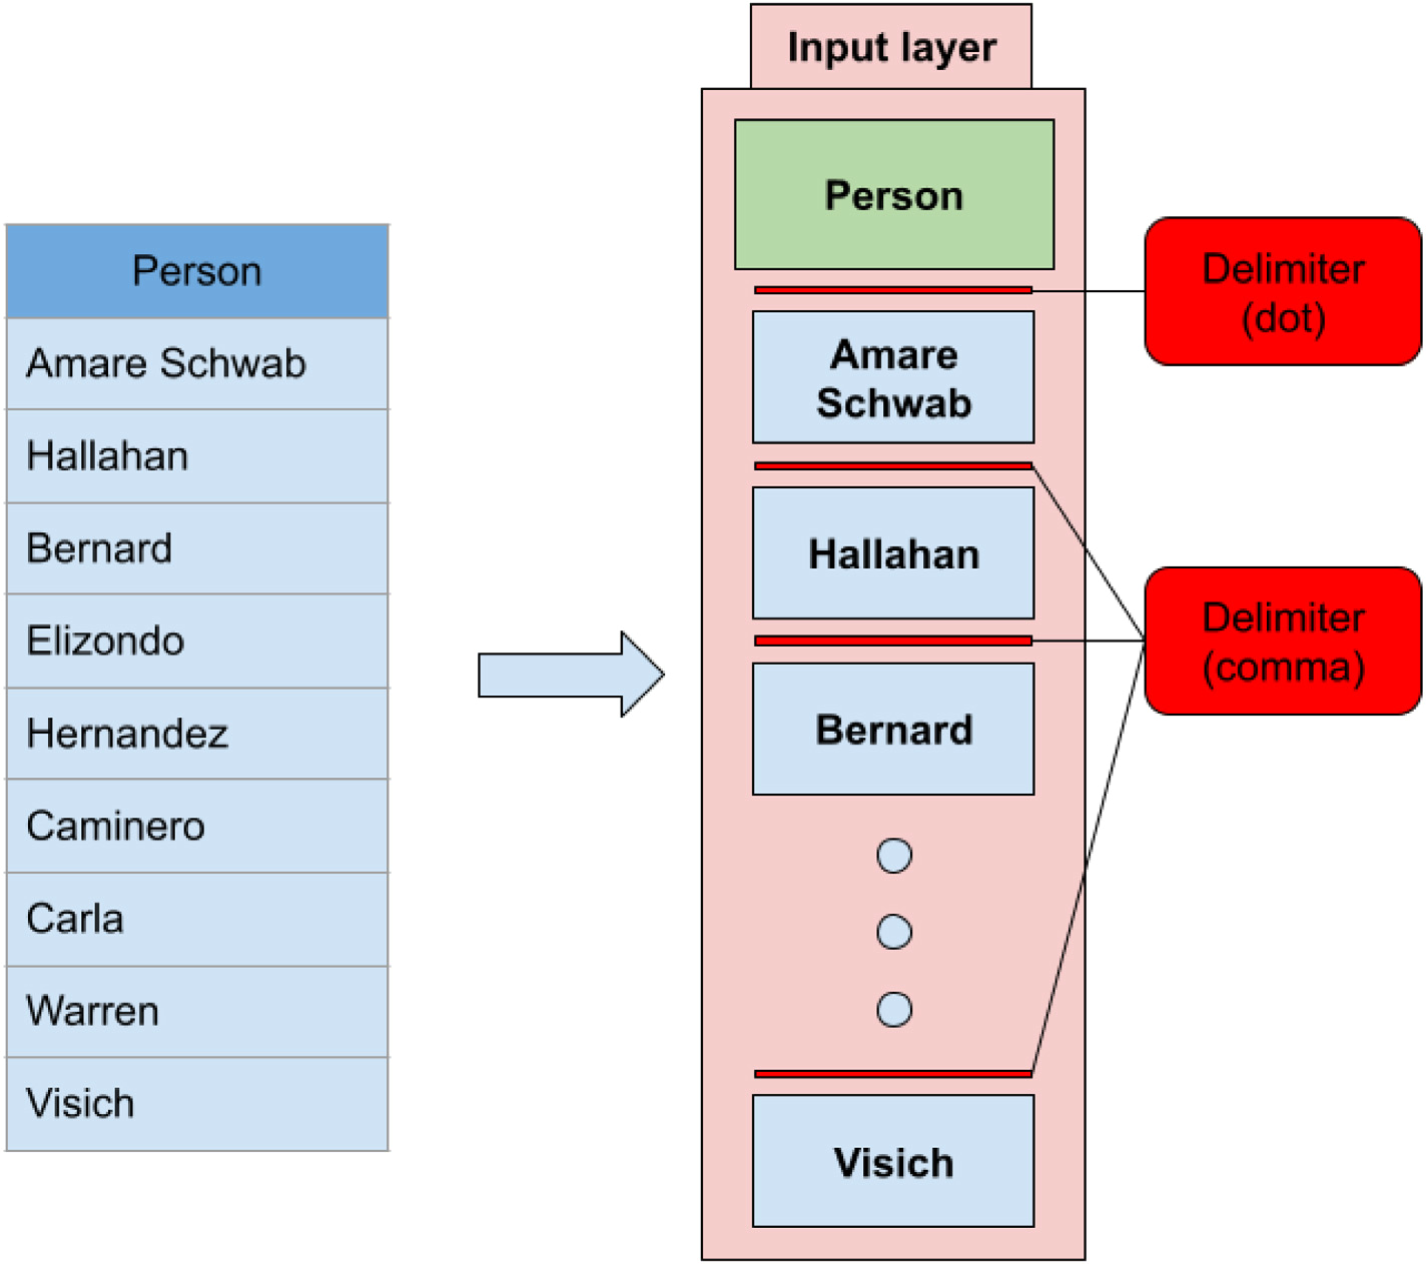
\includegraphics[width=0.8\linewidth]{\figdir/cassed_input.png}
    \caption{Beispiel einer Umwandlung einer Spalte in einen Input-Vektor. Quelle: \cite{Kuzina.2023}.}
    \label{f:input}
\end{figure}

Für die Klassifizierung generiert der Decoder von BERT für jede potenzielle Klasse eine nicht normalisierte Vorhersage. Diese Vorhersagen werden dann über alle Teile der Spalte gemittelt, in die die Spalte aufgeteilt wurde. Anschließend wird eine Sigmoidfunktion auf die Vorhersagewerte angewendet, um normalisierte Wahrscheinlichkeiten für jede Klasse zu erzeugen.

Der CASSED-Ansatz enthält neben dem BERT-Modell auch eine regelbasierte Schicht, die strukturierte Formate wie E-Mails oder Sozialversicherungsnummern mittels regulären Ausdrücken klassifiziert. Zudem wird ein Wörterbuch für bekannte sensible Daten oder Merkmale von Geschäftsgeheimnissen verwendet. Auch diese Schicht ermittelt für jede Klasse eine mögliche Wahrscheinlichkeit. Die Wahrscheinlichkeiten der regelbasierten Schicht und der BERT-Schicht werden kombiniert, um eine Gesamtwahrscheinlichkeit pro Klasse zu erhalten. Anschließend werden den Daten jene Klassen zugeteilt, deren Wahrscheinlichkeit einen festgelegten Schwellwert überschreitet. Es besteht somit die Möglichkeit, dass einer Datenbankspalte mehrere Klassen zugeordnet wird. Die Architektur des CASSED-Ansatzes wird in \ref{f:cassed} dargestellt.

\begin{figure}[htbp]
    \centering
    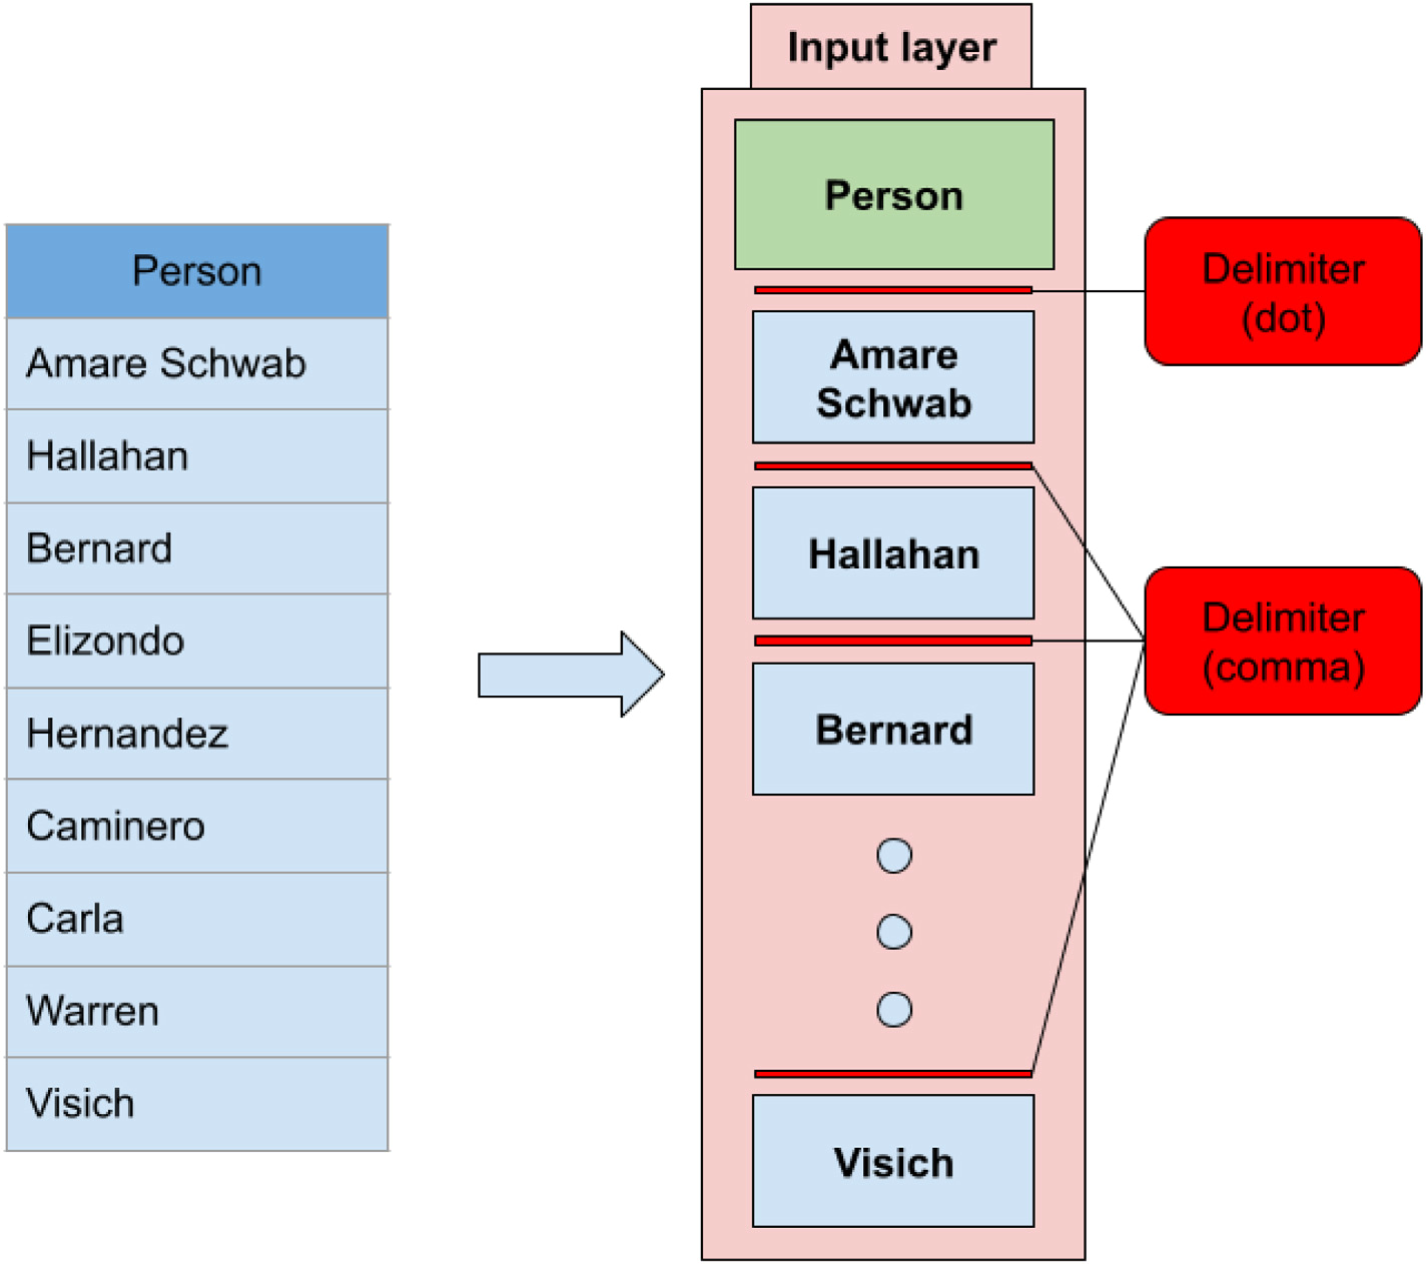
\includegraphics[width=\linewidth]{\figdir/cassed_model.png}
    \caption{Überblick über die CASSED Methode. Quelle: \cite{Kuzina.2023}.}
    \label{f:cassed}
\end{figure}

Die CASSED-Methode zeigt im Vergleich zu anderen kontextbasierten Klassifizierungsmethoden deutlich bessere Ergebnisse. Das Modell erzielt nicht nur bessere Leistungen durch den alleinigen Einsatz von BERT, sondern wird durch die Integration der regelbasierten Schicht noch präziser.

Guo, Liu et al. \cite{Guo.2021} verfolgen einen ähnlichen Ansatz mit ihrem Modell 'Exsense'. Auch sie verwenden zwei Schichten: eine inhaltsbasierte Analyse mit regulären Ausdrücken und eine kontextbasierte Analyse mit einem BERT-BiLSTM-Attention-Modell. Dabei wird das BERT-Modell kombiniert mit einem Bidirectional Long Short-Term Memory Modell (BiLSTM). BiLSTM ist ein rekurrentes neuronales Netzwerk, das für die Verarbeitung von sequenziellen Daten entwickelt wurde und sich gut zur Erfassung von Abhängigkeiten in langen Sequenzen eignet. Im BERT-BiLSTM-Modell dient die bidirektionale Kontextrepräsentation von BERT als Eingabe für das BiLSTM. Dieser Ansatz zeigt ebenfalls herausragende Ergebnisse bei der Klassifizierung sensibler Daten unter Berücksichtigung des Kontextes.

Insgesamt zeigen alle vorgestellten Klassifizierungsmethoden aus dem KI-Bereich sehr gute Ergebnisse bei der Klassifizierung von sensiblen Daten.

% ###########################################
% \paragraph{TF-IDF}
%'Term Frequency' und 'Inverse Document Frequency' (TF-IDF) ist eine häufiger verwendete Technik, bei der die Bedeutung eines Begriffs direkt proportional zur Häufigkeit des Auftretens des Begriffs in einem Dokument ist und umgekehrt proportional zur Häufigkeit des Auftretens des Begriffs im gesamten Dokument ist. Diese Technik wird häufig in verschiedenen Bereichen wie Data Mining oder Textklassifizierung eingesetzt.

% ###########################################
\subsection{Anwendung in der Cloud Security}
% wofür ist das dann gut
Wie in Kapitel \ref{dlp-kapitel} erläutert, spielt die Datenklassifikation eine entscheidende Rolle in DLP-Systemen. Das automatische Erkennen und Klassifizieren sensibler Daten ist ein zentraler Bestandteil dieser Systeme, da Sicherheitsmaßnahmen und -techniken auf der Kenntnis über die Sicherheitsstufen der Daten basieren.
Ein Beispiel für ein solches Cloud-DLP-System ist der Google Cloud Data Loss Prevention Service. Dieser vollständig verwaltete Dienst ermöglicht Unternehmen die Erkennung, Klassifizierung und den Schutz sensibler Daten in Cloud- und lokalen Umgebungen. Der Dienst nutzt maschinelles Lernen und Mustervergleichstechniken, um bis zu 150 verschiedenen Datentypen zu identifizieren und entsprechend zu klassifizieren. Durch diese Klassifizierung können dann im Cloud-DLP-System unterschiedliche Schutzmaßnahmen für verschiedene Datentypen und Klassen festgelegt werden \cite{GoogleCloud.30.11.2023}.

Ein weiteres Beispiel ist das Software-Produkt Digital Guardian Cloud Data Protection des Anbieters Fortra. Das Cloud-DLP-System umfasst verschiedene Module, wobei eines davon die Datenklassifizierung ist. Dieses Modul identifiziert und klassifiziert sensible Daten und hängt ihnen verschiedene Sicherheitsstufen-Labels an. Die Klassifizierung erfolgt dabei automatisch auf Grundlage von Inhalt und Kontext. Zudem besteht die Möglichkeit, eine manuelle Klassifizierung durch den Benutzer vorzunehmen. Das Cloud-DLP-System von Fortra ist dabei mit allen führenden Cloud-Plattform-Anbietern kompatibel \cite{DigitalGuardian.30.11.2023}.

Die Klassifizierung und die Markierung der Daten dient in Cloud-DLP-Systemen anschließend dazu, geeignete Schutzmaßnahmen zu definieren. Im Folgenden werden verschiedene Techniken beschrieben, die eine versehentliche Offenlegung von sensiblen Daten verhindern.

% Wasserzeichen
Eine der ersten Techniken zum Schutz von sensiblen Daten ist die Wasserzeichen-Methode. Dabei werden spezifische Identifikationsmerkmale oder Muster durch einen Algorithmus in Daten eingebettet, um die Quelle oder den Eigentümer zu kennzeichnen. Wasserzeichen dienen dazu, den Ursprung von Daten zu verfolgen und zu überwachen, um unbefugte Verbreitung oder Weitergabe zu erkennen. Systeme können anhand der eingebetteten Wasserzeichen erkennen, wenn Daten ohne Berechtigung weitergegeben oder veröffentlicht werden, und Maßnahmen ergreifen. Auf diese Weise können Datenlecks und -manipulationen mithilfe von Wasserzeichen erkannt und verhindert werden \cite{Naik.2019}.

%Blacklisting, Whitelisting
Eine weit verbreitete Methode in DLP-Systemen ist das Blacklisting oder Whitelisting. Das Modell besteht aus Regeln, die Muster böswilliger Aktivitäten oder markierte sensible Daten definieren, die das Unternehmensnetzwerk nicht verlassen dürfen. Beim Whitelisting wird definiert, welche Daten geteilt werden dürfen, beim Blacklisting werden die Daten und Muster definiert, die nicht geteilt werden dürfen. So kann ein DLP-System anhand dieser Regeln und Listen Transaktionen blockieren und somit eine versehentliche Offenlegung von sensiblen Daten verhindern. Allerdings ist es für böswillige Insider oft leicht, eine Blacklisting-basierte Erkennung zu umgehen, da je nach Berechtigungen die Regeln und Listen bekannt sind \cite{Costante.2016}.

% Verschlüsselung
Die Kryptografie ist eine häufig verwendete Technik im Datenschutz. Sie wandelt Informationen von einem lesbaren Format in ein verschlüsseltes Format um. Je nach Sicherheitsstufe der Daten können unterschiedliche Verschlüsselungsalgorithmen und kryptografische Funktionen zum Einsatz kommen \cite{HerreraMontano.2022}. Dabei ist es nicht sinnvoll, einfach alle vorhandenen Daten verschlüsselt zu speichern oder zu übertragen. Insbesondere bei großen Datenmengen kann das schnell zu Performance-Problemen führen. Die Verschlüsselung von Daten erfordert Rechenressourcen und erhöhten Speicherbedarf. Deshalb wird meistens nur nach Bedarf verschlüsselt \cite{Arki.2023}.
Zardari, Jung et al. \cite{Zardari.2014} kategorisieren in ihrem vorgeschlagenen Modell Daten nach sensibel und nicht-sensibel. Nicht-sensible Daten werden direkt im Cloud-Speicher gespeichert, sensible Daten werden vorher mit dem RSA-Algorithmus verschlüsselt.

% Hashing
Das Fingerprinting-Verfahren, das im Kapitel \ref{fingerprint} zur automatischen Klassifizierung beschrieben wurde, kann auch als Schutzmaßnahme dienen. Mit einem Vergleich von Datei- oder Daten-Hashes kann der ausgehende Datenverkehr überwacht werden. Ein DLP-System gleicht dabei die Hashes der Daten im Datenverkehr mit denen der als sensibel markierten Daten ab und kann so bei Übereinstimmung ein Datenleck erkennen und verhindern. Auch hier ist die Wahl des Hashing-Verfahrens relevant, wie verlässlich auch veränderte Daten noch erkannt werden \cite{HerreraMontano.2022}.

% Cloud Shredder
Zhang, Jing et al. \cite{Zhang.2011} stellen eine Methode vor, um die versehentliche Offenlegung von sensiblen Daten zu verhindern, selbst wenn bspw. ein ungeschützter Laptop verloren geht. Der Ansatz namens 'Cloud Shredder' sieht vor, dass vertrauliche Dateien geschreddert, also in Stücke geteilt wird. Ein Teil wird auf dem physischen Gerät und ein Teil im Cloud-Speicher gespeichert. Nur wer Zugriff auf beide Bereiche hat, kann die sensiblen Dateien lesen oder verarbeiten.

% DocGuard
Ein weiterer Ansatz namens 'DocGuard' wurde von Gui, Puzis et al. in \cite{Guri.2019} vorgestellt. Die Idee besteht darin, dass bereits vorhandene Antiviren-Software durchgesickerte Daten identifiziert und den Zugriff blockiert. Das funktioniert, indem DocGuard bei sensiblen Daten eine versteckte Signatur einer bekannten Schadsoftware einfügt. Wenn diese Daten das Unternehmensnetzwerk verlassen, erkennt eine Antiviren-Software die schadhafte Signatur als Bedrohung und greift ein.

% BrowserFlow
In Unternehmen werden externe Cloud-Dienste wie Google Docs vermehrt genutzt. Dabei können Benutzer schnell gegen unternehmensinterne Daten-Richtlinien verstoßen. Sensible Daten sind leicht aus einem geschützten Cloud-Dokument in ein ungeschütztes Cloud-Dokument kopiert und damit offengelegt. Papagiannis, Watcharapichat et al. \cite{Papagiannis.2016} schlagen als Lösung für dieses Problem ihren Ansatz namens 'BrowserFlow' vor. BrowserFlow ist eine browserbasierte Middleware, die Datenflüsse verfolgt, indem sie die Ähnlichkeit zwischen Textfragmenten erkennt. Anhand von gekennzeichneten Daten können so nicht autorisierte Datenflüsse identifiziert und verhindert werden.

Es zeigt sich also, dass es viele verschiedene einfache und aufwändigere Methoden in der Cloud Security gibt, um sensible Daten zu schützen. Die Zuverlässigkeit dieser Methoden basieren auf der Qualität der Klassifizierung. Deshalb ist eine automatische Klassifizierung mit bewährten KI-Verfahren eine gute Wahl und immer häufiger in DLP-Systemen im Einsatz.
